\section{Regular implies $\CMSO$ definable}\label{sec:reg->def}


\begin{theorem}\label{thm:reg->MSO}
If a language is regular, then it is $\CMSO$ definable. 
\end{theorem}

To prove Thm.~\ref{thm:reg->MSO}, we proceed by induction on  regular expressions. The cases of word and multiset regular expressions follow from the similar result for words and commutative words. The cases of union and the operations of the signature $\sigma$ follow from Prop.~\ref{prop:CMSO-def-operations}. We are left with the cases of substitution and iteration; the rest of this section is dedicated to proving the following proposition.
 
\begin{proposition}\label{prop:Guarded-It-Is-CMSO}
Let $x$ be a letter and $L$ and $M$ be languages of $\TWT$ graphs. We have:
$$
\begin{array}{ccc}
\text{$M [L/x]$ is guarded and $L$ and $M$ are $\CMSO$-definable} & \Rightarrow & \text{$M[L/x]$ is $\CMSO$-definable.}\\[3pt]
\text{$\mu x. L$ is guarded and $L$ is $\CMSO$-definable} &\Rightarrow& \text{$\mu x. L$ is $\CMSO$-definable.}
\end{array}$$
\end{proposition}


We handle the case of iteration, the case of substitution being similar. We show first that the iteration of a $\CMSO$ definable language, without any guard condition, is definable in an extension of $\CMSO$ where we are allowed to quantify existentially over sets of subgraphs of the input graph, which we call $\CMSOd$. This logic is obviously strictly more expressive then $\CMSO$, because it amounts to quantify over sets of sets. Based on this, we show that the  \emph{guarded iteration} of a $\CMSO$ definable language is  definable in $\CMSO^r$, the extension of $\CMSO$ with companion relations defined in the previous section. This concludes the proof, the logic $\CMSO^r$  being equivalent to $\CMSO$.



\subsection{Iteration of $\CMSO$ formulas is $\CMSOd$ definable}

\subsubsection{Decompositions}

When a graph is in the iteration $\mu x. L$ of some language $L$, it is possible to structure it into a tree shaped decomposition, such that each part of this decomposition ``comes from $L$''. In the following, we define such decompositions.  


\begin{definition}[Independent graphs] 
Let $G$ be a graph and $H, K$ be subgraphs of $G$.  We say that $H$ and $K$ are \emph{independent} if they do not share any edge; and whenever they share a vertex, it is necessarily an interface vertex of both $H$ and $K$. 
\end{definition}
\begin{remark}
Two independent subgraphs can share at most two vertices.
\end{remark}
\begin{definition}[Decompositions]
A \emph{decomposition} of $G$ is a set $\cD$  of modules of $G$ such that  $G\in \cD$ and for every pair of  graphs in $\cD$, they are either independent, or module one of the other. We call  the graphs of  a decomposition its \emph{components}. We call \emph{the interfaces of $\cD$} the set of interfaces of its components. 
\smallskip

Let $H$ and $K$ be components of a decomposition $\cD$. We say that $H$ is a \emph{child} of $K$, if $H$ is a module of $K$, and if there is no component $C$ of $\cD$, distinct from $H$ and $K$,  such that $H$ is a module of $C$ and $C$ is a module of $K$. 
\smallskip

The graph $G$ is called the \emph{head} of $\cD$. A component of $\cD$ is a \emph{leave} if it does not contain another component of $\cD$ as a module.
 \end{definition}
 \begin{remark} Note that  the children of a component are pairwise independent.
\end{remark}


 \begin{example}\label{example:decomposition} Let $G$ be the left graph below. The right picture is a decomposition of $G$, where the child relation  is materialized by the dotted lines. The colors have no specific meaning here, but will be useful to illustrate the upcoming notion of the \emph{components body}.  
 \begin{center}
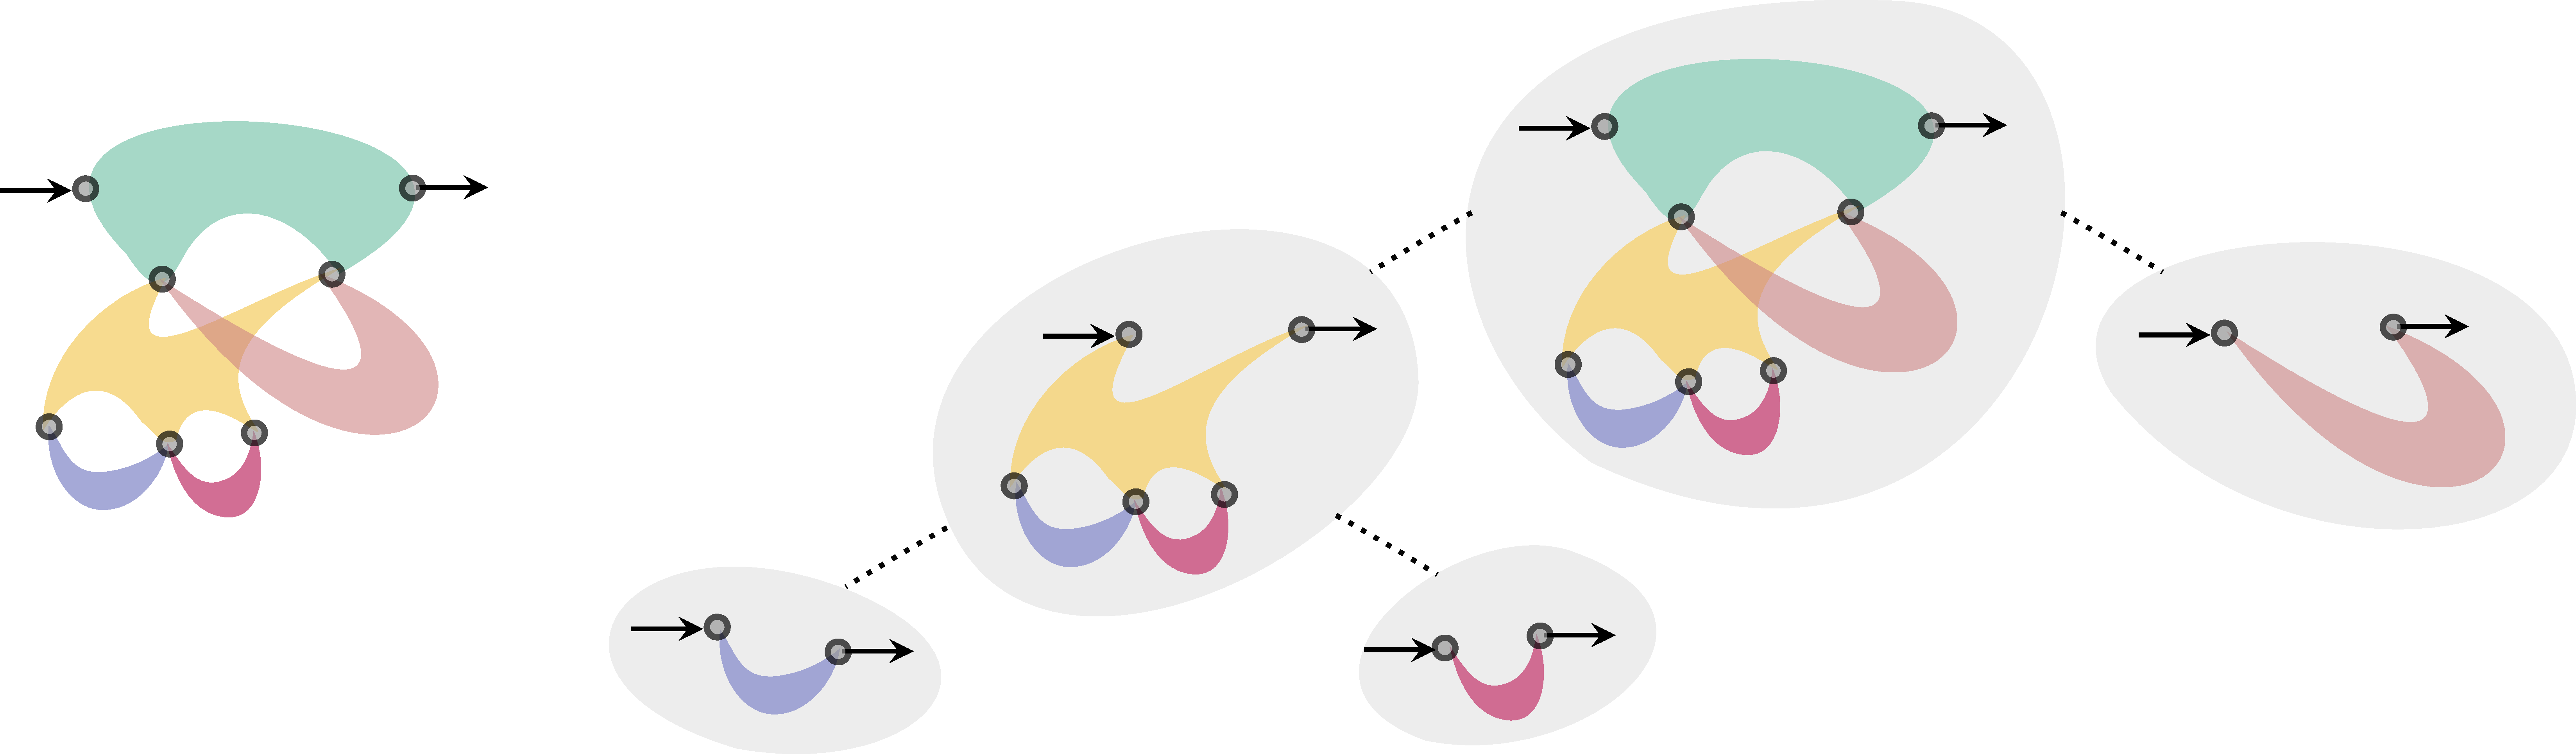
\includegraphics[scale=.10]{Pictures/decomposition}
\end{center}
 \end{example}
 
 \begin{definition}[Body of a component]
Let $G$ be a graph, $\cD$ a decomposition of $G$ and $C$ a component of $\cD$. 
\smallskip

The \emph{body} of $C$ is the subgraph of $G$ whose vertices are those of $C$ minus the \textbf{inner} vertices of its children; and whose edges are those of $C$ minus those of its children.  
\smallskip

The \emph{$x$-body of $C$} is the graph whose interface is the interface of $C$, whose vertices are the vertices of the body of $C$, and whose edges are the edges of the body of $C$ plus, for each child $F$ of $C$, an $x$-edge whose interface is the interface of $F$.  We denote it  by $x\text{-}\mathsf{body}_\cD(C)$.
\end{definition}

\begin{definition}[$L$-decompositions]
Let $L$ be a graph language. An $L$-decomposition of a graph $G$ is a decomposition of $G$ such that the $x$-body of each of its components is in $L$.
\end{definition}

\begin{example}
Below, from left to right, a component of the decomposition of Ex.~\ref{example:decomposition}, its body, and its $x$-body. Actually, each monochromatic subgraph of $G$ corresponds to the body of a  component of this decomposition.
\begin{center}
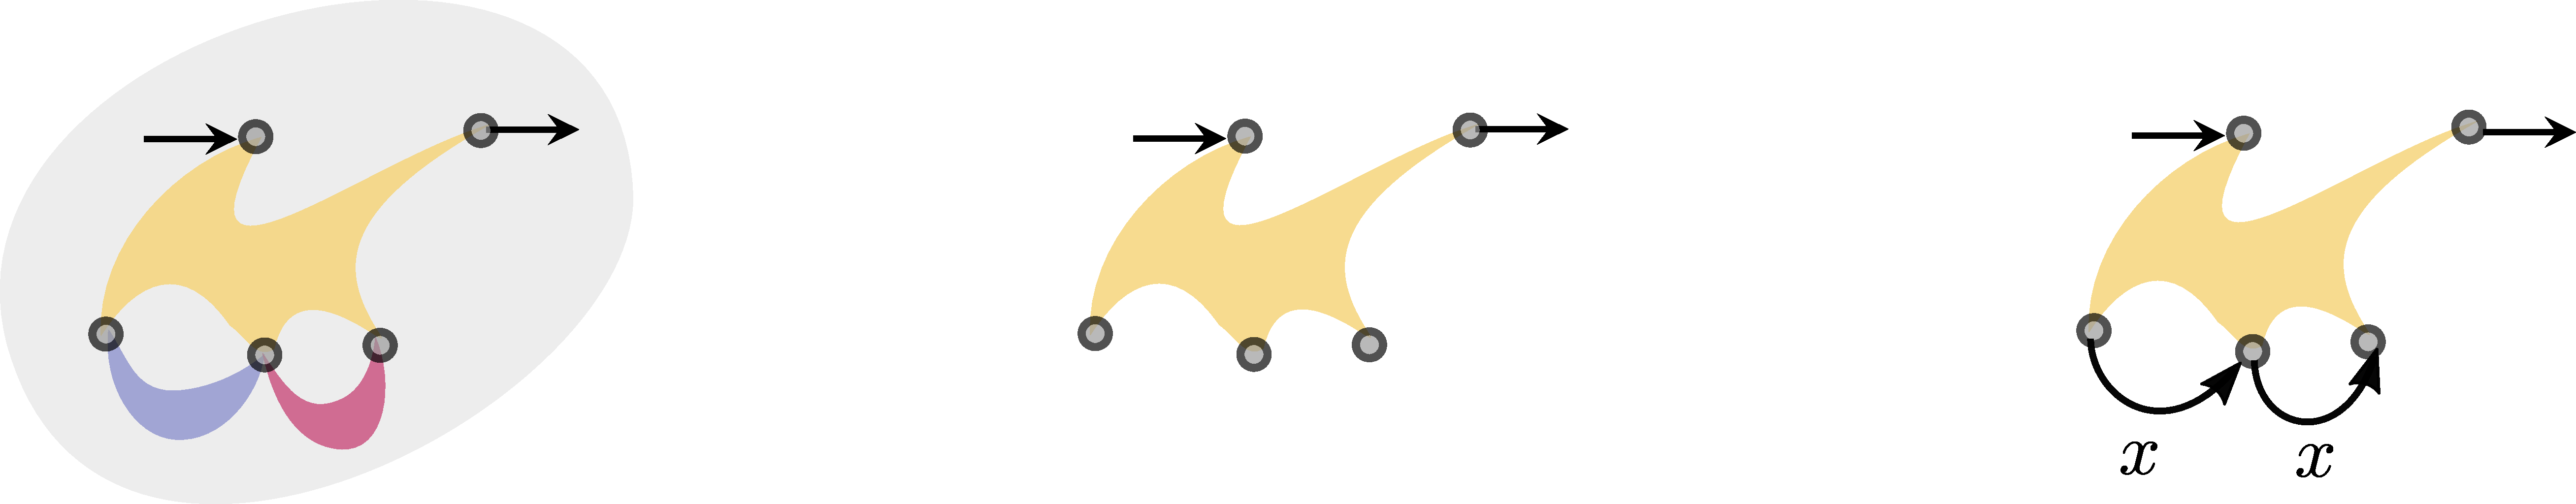
\includegraphics[scale=.10]{Pictures/body}
\end{center}
\end{example}
\begin{remark}
The body of a component is a subgraph of $G$, but its $x$-body is not a subgraph of $G$ in general, because of the added $x$-edges.
\end{remark}


 

\begin{proposition}\label{lem:decomp-iteration}
Let $L$ be a graph language. We have:
$$ G\in \mu x. L \qquad \Leftrightarrow \qquad \exists \cD. \ \quad\cD \text{ is an $L$-decomposition of $G$.}$$
\end{proposition} 
The proof of this proposition is based on the following easy lemma:

\begin{lemma}\label{lem:decomp-one-step}
Let $L$ be a language, $G, G_1,\dots, G_k$ be graphs and $H$ a $k$-context satisfying:
 $$G=H[G_1,\dots, G_k]\qquad\text{ and }\qquad H[x,\dots,x]\in L$$
Let $\cD_i$ be an $L$-decomposition for $G_i$, for $i\in [1,k]$, and let $\cD$ be the following set
 $$\cD:=\cD_1\cup \dots\cup \cD_k\cup\set{G}.$$
 The set $\cD$ is an $L$-decomposition of $G$.
\end{lemma}

\begin{proof}[Proof of Prop.~\ref{lem:decomp-iteration}]
We show by induction on $n\in\mathbb{N}$, that the  property $P_n$ is true:
$$\begin{array}{lrll}
P_n:&\qquad\forall G.\ \quad G\in L^{n,x}& \Rightarrow& \exists \cD. \ \quad\cD \text{ is an $L$-decomposition of $G$.} 
\end{array}
$$
The base case is trivial, and the inductive case is based on Lemma~\ref{lem:decomp-one-step}.
\end{proof}



\subsubsection{The logic $\CMSOd$}
Let $\phi$ be a $\CMSO$ formula defining a graph language $L$. Using Prop~\ref{lem:decomp-iteration}, we can express that a graph $G$ is in the iteration $\mu x. L$ by guessing a decomposition $\cD$ of $G$, and ensuring that the $x$-body of each component  satisfies $\phi$.   But guessing a set of subgraphs is not expressible in $\CMSO$. This is why we introduce $\CMSOd$, an extension of $\CMSO$ where this is allowed. 


\begin{definition}[$\CMSOd$ logic] Let $\mathbb{X}_d$ be a set of \emph{graph set variables}, whose elements are denoted $\cX, \cY\dots$. The formulas of $\CMSOd$ are of the following form:
\begin{align*}
 \phi :=&\ \CMSO\ |\ \exists \cX.\ \phi\ |\ (s,Z,t)\in \cX & \qquad (\cX\in \mathbb{X}_d, \ \ Z\in \mathbb{X}_2,\ \  s,t\in\mathbb{X}_1).
\end{align*}
\end{definition}
Free and bound variables are defined as usual.  As for $\CMSO$, we need to define the semantics of a formula over pointed graphs to handle free variables. 

\begin{definition}[Semantics of $\CMSOd$] Let $G$ be a graph and $\Gamma$ be a set of variables.  

An \emph{interpretation of $\Gamma$} is a function mapping every first-order variable of $\Gamma$ to an edge or vertex of $G$, every set variable to a set of edges and vertices of $G$, and every graph set variable to a set of subgraphs of $G$.    

We define the \emph{satisfiability relation} $\langle G, I\rangle\models \phi$ as usual, by induction on  $\phi$. The only new cases compared to $\CMSO$ are the quantification  $\exists \cX$ which is interpreted as ``there exists a set of subgraphs $\cX$'', and the formulas $(s,Z,t)\in \cX$ which are interpreted as ``the graph whose input is $s$, whose output is $t$ and whose set of edges and vertices is $Z$, is an element of $\cX$''.  
\end{definition}
\begin{proposition}\label{prop:def-decomp}
There is a $\CMSOd$ formula $\mathsf{decomp}(\cX)$, \emph{without graph set quantification}, such that for every graph $G$ and every set of subgraphs $\cD$ of $G$, we have:
\begin{align*}
\qquad\qquad\qquad\langle G, \cX\mapsto \cD\rangle\models \mathsf{decomp}(\cX)\quad \Leftrightarrow \quad  \cD \text{ is a decomposition of } G.
\end{align*}
\end{proposition}
\begin{proof} 
We can express in $\CMSOd$ that a graph is a module of another graph using Prop.~\ref{prop:pure-modules-are-CMSO}. We can express that two graphs $(s,Z,t)$ and $(s',Z',t')$ are independent using the following formula:
$$ (x\in Z\  \wedge\  x\in Z')\ \ \Rightarrow (x=s\  \vee\  x=s'\  \vee\  x=t\ \vee\ x=t')$$
 This is how we express that $\cX$ is a decomposition. Note that we do not need to introduce a  quantification on new graphs set variables. 
\end{proof}


\subsubsection{Iteration is expressible in $\CMSOd$}

Given a $\CMSO$ formula $\phi$, we construct a formula $\tms{\phi}$ having $\cX$ as unique free variable, which expresses the fact that the $x$-body the head of the decomposition $\cX$ satisfies $\phi$. To construct $\tms{\phi}$, we need the following definition.

\begin{definition}[Complete sets] Let $\cD$ be a decomposition of a graph $G$. 
\smallskip

Let $H$ be a set of edges and vertices of $G$. We say that $H$ is \emph{complete} if, whenever it contains an edge or an inner vertex of a child $C$ of $G$ (seen as a component of $\cD$), then it contains all the edges and  inner vertices of $C$. 
\smallskip

Let $K$ be a set of edges and vertices of the $x$\text{-}body of $G$.  We denote by $\mathsf{complete}_\cD(K)$ the set of edges and vertices of $G$,  obtained from $K$ by replacing every $x$-edge coming from a child $C$ of $G$  by the set of edges and inner vertices $C$.  
\end{definition}
\begin{remark}
Note that if $H$ is complete, there is a set $S$ such that $H=\mathsf{complete}_\cD(S)$.
\end{remark}

Here is a picture illustrating complete sets. The green part is the body of $G$ and the purple modules are its children. The yellow sets are complete, but the pink one is not. 
\begin{center}
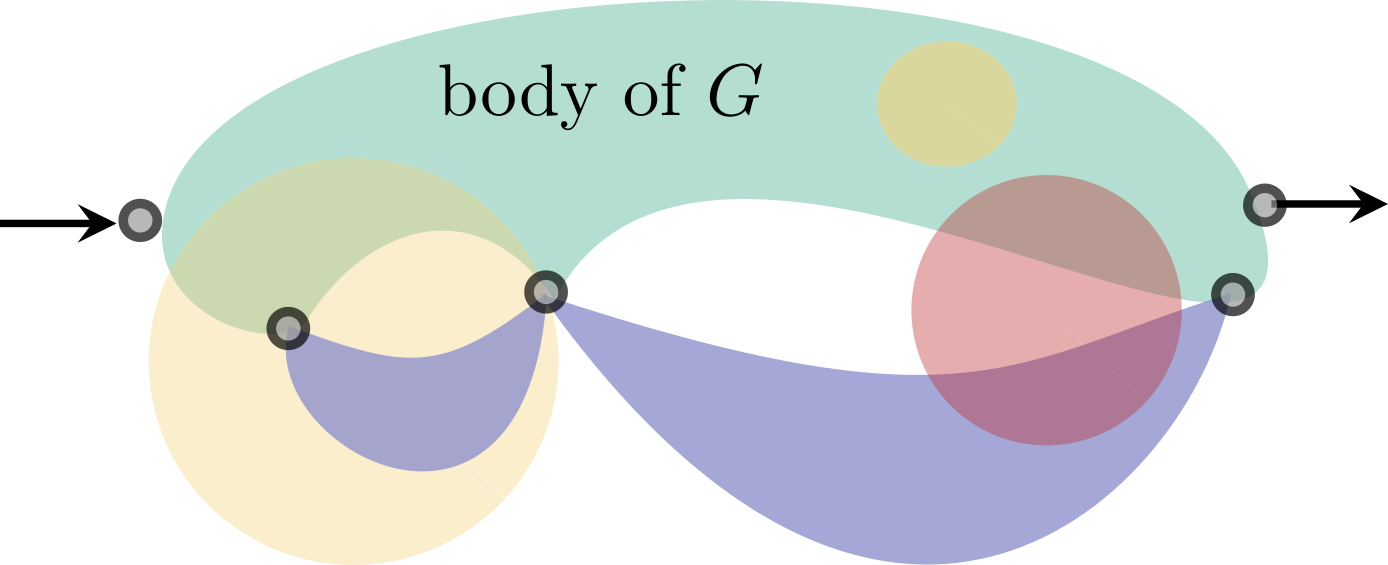
\includegraphics[scale=.12]{Pictures/complete-set}
\end{center}

\begin{proposition}
The following  formulas are  $\CMSOd$ definable:
\smallskip

\begin{tabular}{lrp{11cm}}
 $\mathsf{child}_\cX(Y)$&:&  $Y$ is the set of edges and inner vertices of a child of the input graph w.r.t. the decomposition  $\cX$.\\[4pt]
 $\mathsf{is\text{-}complete}_\cX(Y)$&:&  $Y$ is complete wrt $\cX$.\\[4pt]
 $\mathsf{body\text{-}edge}_\cX(Y)$&:& $Y$ is a singleton containing an edge from the body of the input graph wrt $\cX$.\\[4pt]
 $\mathsf{source}_\cX(Y,Z)$&:& $\mathsf{child}_\cX(Z)$ and $Y$ is a singleton containing the input of the corresponding child. \\[4pt]
 $\mathsf{target}_\cX(Y,Z)$&: &the same as above, where input should be replaced by output.\\[4pt]
  $\mathsf{choice}_\cX(Y,Z)$&: & $Z$ contains all the body elements of $Y$, and for every child contained in $Y$, $Z$ contains exactly one element of this child.
\end{tabular}
\end{proposition}
%\begin{proof}\todo{complete}
%Faire le cas child et choice qui est le plus interessant. 
%\end{proof}
%\begin{remark}
%Pour construire $\mathsf{choice}_\cX(Y,Z)$, nous avons besoin que les elements de la decomposition ne soient pas vides. 
%\end{remark}
 We construct the formula $\tms{\phi}$ by induction on the structure of $\phi$. We suppose that $\phi$ is build using the syntax of $\CMSO$ where only set variables are allowed.

\begin{definition}\label{def:transfer}  Let $\phi$ be a $\CMSO$ formula whose free variables are $\Gamma$. 
 We define the $\CMSOd$ formula $\tms{\phi}$, whose free variables are $\Gamma\cup\set{\cX}$,  by induction as follows:
 $$\begin{array}{lll}
    \tms{\phi\vee \psi}&= & \tms{\phi} \vee \tms{\psi} \\[4pt]
    \tms{\neg \phi}&= & \neg \tms{\phi}\\[4pt]
      \tms{(|Y|\equiv k)[m]}&= & \exists Z.\ \mathsf{choice}_\cX(Y,Z)\wedge (|Z|\equiv k)[m]\\[4pt]
   \tms{Y\subseteq Z}&= & Y\subseteq Z \\[4pt]
     \tms{a(Y)}&= & a(Y)\qquad (a\neq x) \\[4pt]
       \tms{x(Y)}&= & \mathsf{child}_\cX(Y) \vee (\mathsf{body\text{-}edge}_\cX(Y)\wedge x(Y) ) \\[4pt]
        \tms{\exists Y.\ \phi}&= &\exists Y.\ \mathsf{is\text{-}complete}_\cX(Y)\wedge \tms{\phi}\\[4pt]
 \tms{\mathsf{source}(Y,Z)}& =&(\mathsf{body\text{-}edge}_\cX(Z)\wedge \mathsf{source}(Y,Z) )\vee (\mathsf{child}_\cX(Z)\wedge \mathsf{source}_\cX(Y,Z) )\\[4pt]
 \tms{\mathsf{target}(Y,Z)}&= &(\mathsf{body\text{-}edge}_\cX(Z)\wedge \mathsf{target}(Y,Z) )\vee (\mathsf{child}_\cX(Z)\wedge \mathsf{target}_\cX(Y,Z) )
 \end{array}
 $$
 \end{definition}

Transfer results are results of this form: to check that a transformation $\mathsf{f}(G)$ of a structure $G$ satisfies a formula $\phi$, construct a formula $\mathsf{f}^{-1}(\phi)$ that $G$ should satisfy. The proposition below is a transfer result, where the transformation is the $x$-body.

 \begin{proposition}\label{prop:transfer}
Given a $\CMSO$ sentence $\phi$ defining, there is a $\CMSOd$ formula $\tms{\phi}$ having $\cX$ as unique free variable, such that for every graph $G$ and every decomposition $\cD$  of $G$ \emph{whose components are non-empty}:
$$\langle G,\cX\mapsto\cD\rangle \models\tms{\phi}\qquad \Leftrightarrow \qquad  \text{$x$-}\mathsf{body}_\cD(G)\models \phi.$$
\end{proposition}



\begin{proof} We start by the following definition.
\begin{definition} Let  $\cD$ be a decomposition of  $G$ and $I$  an interpretation of the  set variables $\Gamma$ in  the $x$-body of $G$. We define $I_\cD$, the interpretation of $\Gamma\cup\set{\cX}$ in  $G$ as follows.
\begin{align*}
\qquad\qquad \qquad \quad I_\cD:\ \ & \cX \mapsto \cD, \\
      &   Y \mapsto \mathsf{complete}_\cD(I(Y)), \quad Y\neq \cX.
\end{align*} 
\end{definition}
Let $G$ be the left graph below, the purple graphs being its children for a decomposition $\cD$. The right graph is its $x$-body. The right yellow circles represent the interpretation $I$ of the variables $Y$ and $Z$ in the $x$-body. The left yellow circles represent the interpretation $I_\cD$ of these variables in $G$. 
\begin{center}
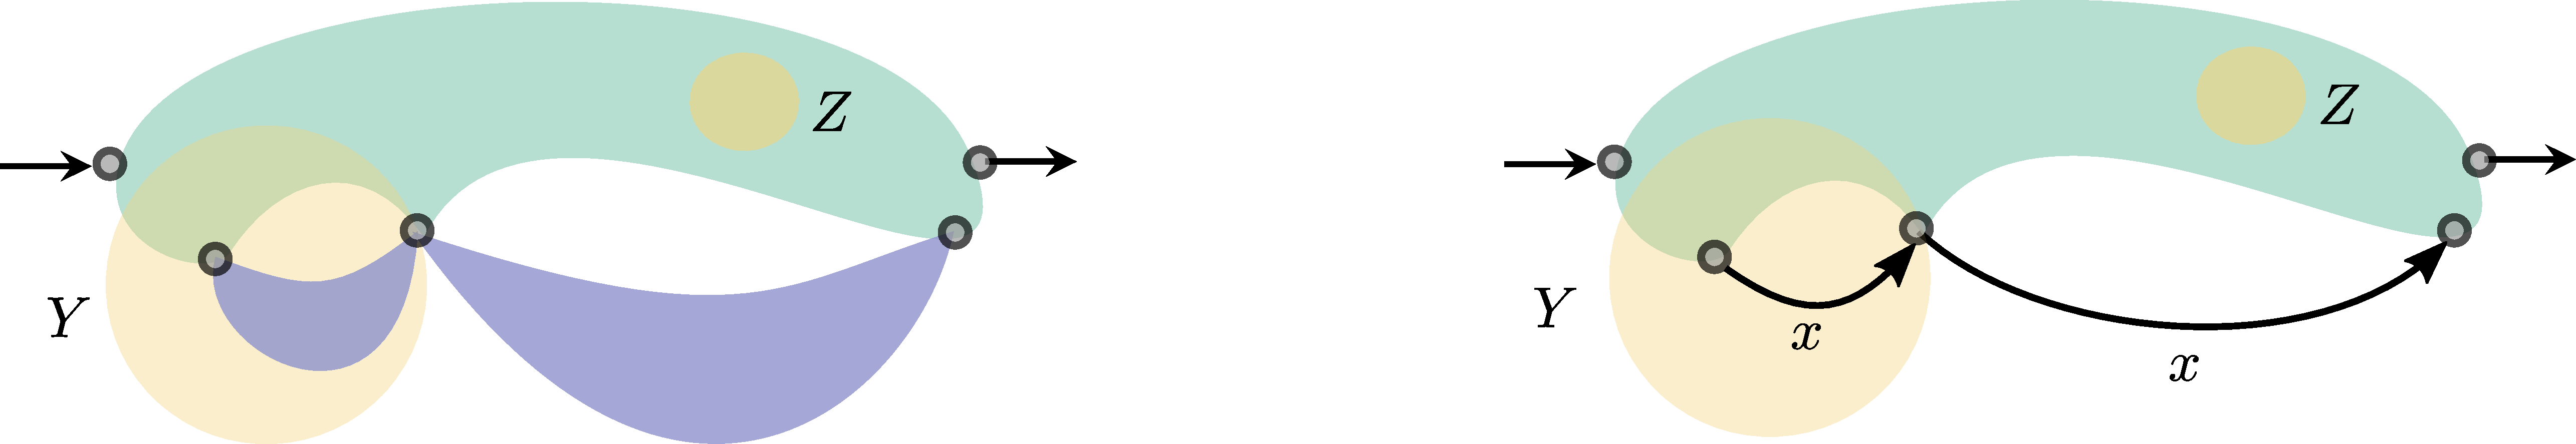
\includegraphics[scale=.12]{Pictures/transfer-interpretation}
\end{center}
The following lemma, which generalizes Prop.~\ref{prop:transfer}, can be proved by a straightforward induction, concluding the proof of this proposition.
 \begin{lemma}
 Let $\cD$ be a decomposition of $G$, $\phi$ a $\CMSO$ formula whose variables are $\Gamma$ and $I$ an interpretation of  $\Gamma$ in the $x$-body of $G$. We have:
 $$ \langle G, I_\cD\rangle \models \tms{\phi} \qquad \Leftrightarrow \qquad\langle x\text{-}\mathsf{body}_\cD(G), I\rangle \models \phi$$ 
 \end{lemma}
We added the non-emptiness condition on the components of $\cD$ to handle the case where $\phi=(|Y|\equiv k)[m]$.
 \end{proof}

The formula  $\tms{\phi}$ expresses the fact that the $x$-body of the head of a decomposition satisfies $\phi$. Using this formula and the localization construction of Prop.~\ref{prop:localization}, we construct a formula $\mu x. L$ saying that the $x$-body of \textbf{all} the components of a decomposition satisfy $\phi$.

\begin{definition}\label{def:iteration}
If $\phi$ is a $\CMSO$ formula, we let $\mu x. \phi$ be the following $\CMSOd$ formula: $$\mu x. \phi:=\ \exists\cX.\ \mathsf{decomp}(\cX)\ \ \wedge\ \ \forall s. \forall Z.\ \forall t.\ (s,Z,t)\in\cX\ \Rightarrow\ \tms{\phi}|_{(s,Z,t)}$$
\end{definition}
The following proposition says that  the language of $\mu x. \phi$ is the iteration of that of $\phi$. 
\begin{proposition}\label{prop:lang-iteration} If $\phi$ is a $\CMSO$ formula defining a language of non-empty graphs, then: $$\ \cL(\mu x. \phi)=\mu x. \cL(\phi).$$
\end{proposition}
\begin{proof} Let $[\phi]$ be the following formula:
$$[\phi]\ :=\ \forall s.\forall Z.\ \forall t.\ \ (s,Z,t)\in\cX\ \Rightarrow\  \tms{\phi}|_{(s,Z,t)}$$  By Prop.~\ref{prop:transfer} and Prop.~\ref{prop:localization}, we can prove the following lemma:
\begin{lemma}
For every graph $G$ and every decomposition $\cD$ of $G$:
$$\langle G,\cX\mapsto\cD\rangle \models[\phi]\qquad \Leftrightarrow \qquad  \forall C\in \cD, \ \text{$x$-}\mathsf{body}_\cD(C)\models \phi.$$
\end{lemma}
We conclude the proof by Prop.~\ref{lem:decomp-iteration}.
\end{proof}

\begin{corollary}
If $L$ is $\CMSO$ definable then  $\mu x. L$ is $\CMSOd$ definable.
\end{corollary}

\subsection{Guarded iteration of $\CMSO$ languages is $\CMSO^r$ definable}

The idea here is that when the iteration $\mu x. L$ is guarded, $L$-decompositions can be encoded by sets of edges and vertices and by companion relations.

\subsubsection{The case of  test languages}
Let $\mu x. L$ be a guarded iteration of type \emph{test}, $G\in \mu x. L$ and $\cD$ an $L$-decomposition of $G$. Suppose that $G$ is the left graph below, and that the red vertices are the interfaces\footnote{Recall that test graphs are unary, hence all the components of a decomposition of $G$ are unary.} of $\cD$.
\begin{center}
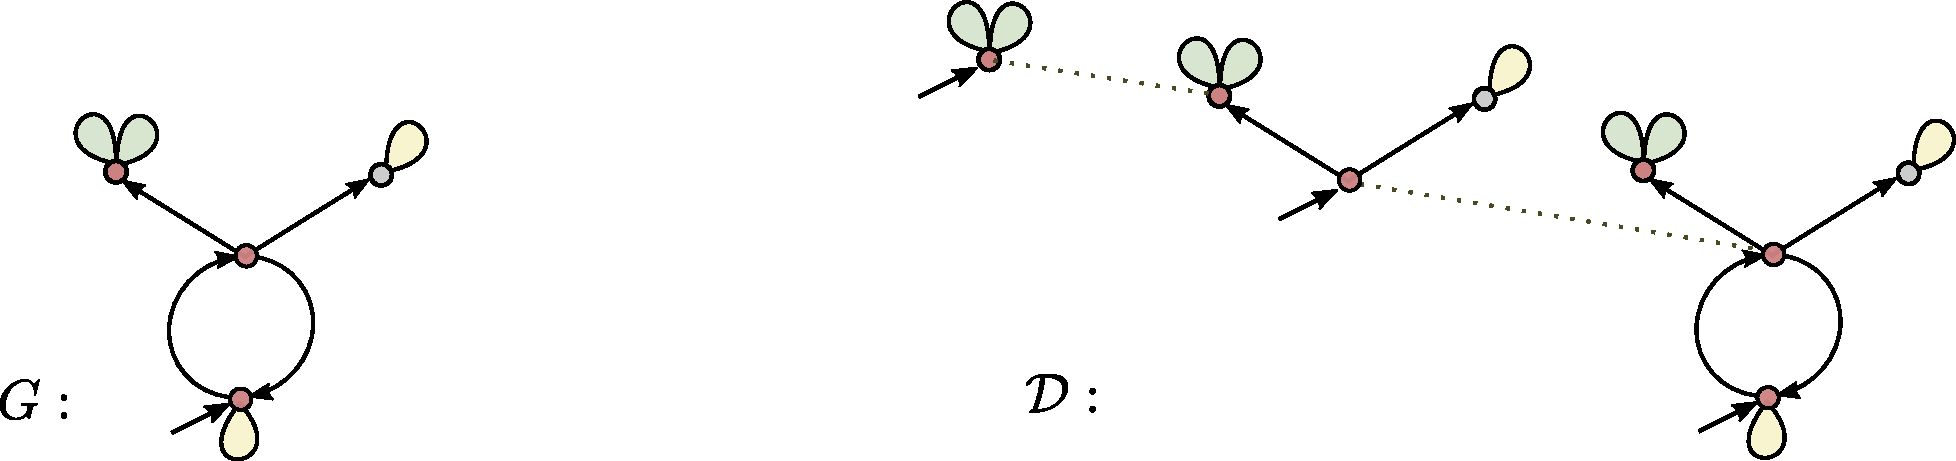
\includegraphics[scale=.33]{Pictures/decomp-test}
\end{center}
We claim that, thanks to the guard condition, this information is enough to reconstruct the whole decomposition $\cD$. More precisely, we claim that the components of $\cD$ are exactly the maximal modules of $G$, whose interfaces are the red vertices, as depicted above.

%This decomposition is depicted above.  By definition, a component of $\cD$ is a module of $G$ whose interface is a red vertex. What we need to show is its maximality. 

%To give an idea for why this should be the case, consider the following decomposition $\cD'$ where one of the components, called $M$, is \textbf{not} a maximal module. Let $H$ be  the $x$-body of $G$ with respect to the decomposition $\cD'$. Notice that  $x$ has a parallel face in $H$, which is not possible because of the guard condition and because  $H\in L$.
%\begin{center}
%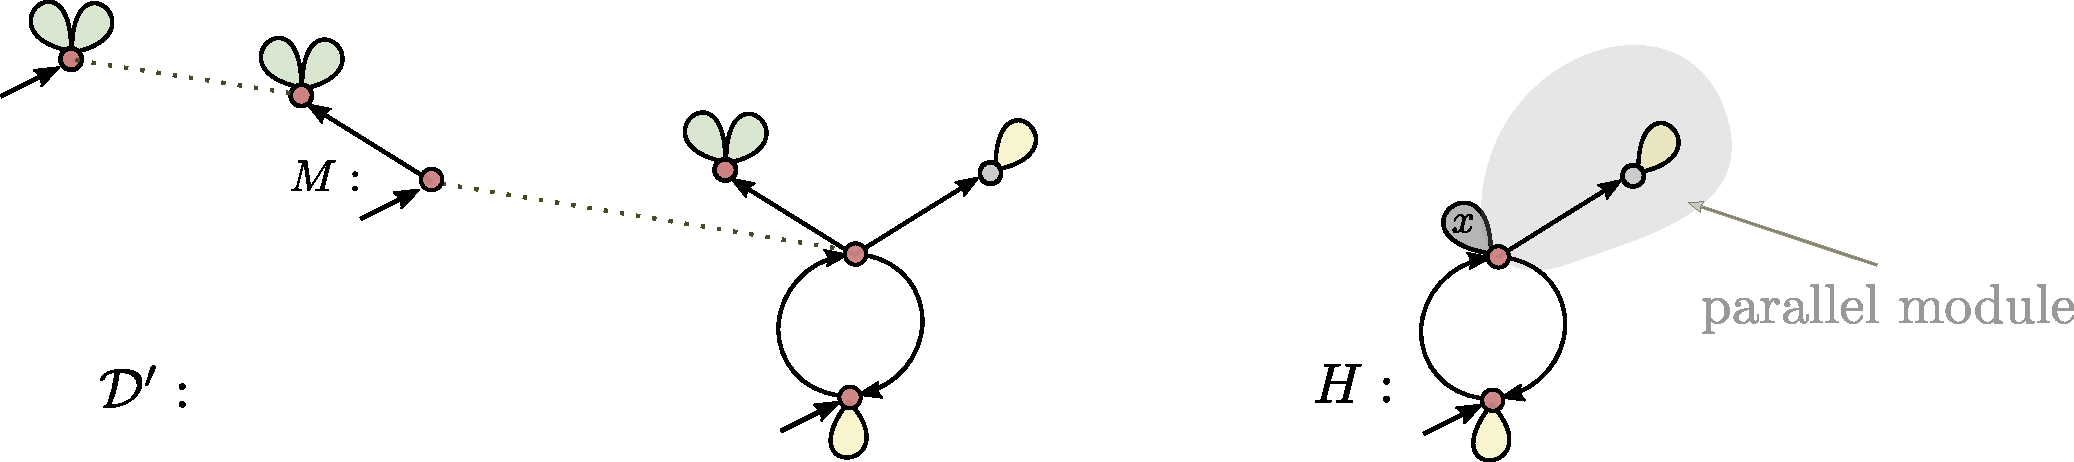
\includegraphics[scale=.4]{Pictures/if-not-max}
%\end{center}
%Our goal will be to make this idea more precise, and this justifies the following definition.
% which associates to a set of vertices of a given graph,  the maximal (unary) modules having these vertices as interfaces.


\begin{definition}  Let $G$ be a graph and $S$ be a set of vertices of $G$.   
We define $\cD_\mathsf{t}(S)$ as the set of maximal modules of $G$, whose type is test, and whose interfaces belong to $S$.  
\end{definition}

\begin{proposition}\label{prop:decomp-iteration-test} Let  $\mu x. L$ be a guarded iteration of type test. We have:
$$\begin{array}{rll}
  G\in \mu x. L& \qquad\Leftrightarrow \qquad\qquad& \exists S.\quad  S \text{ is a set of vertices of $G$ and }\\[3pt]
                      &             & \qquad \ \cD_\mathsf{t}(S) \text{ is an $L$-decomposition of $G$.} 
\end{array}
$$
\end{proposition}

\begin{proof} 
 $(\Rightarrow)$ Follows from Prop.~\ref{lem:decomp-iteration}. To prove  $(\Leftarrow)$, we define the property $P_n$ as follows:
$$\begin{array}{lrll}
P_n:&\qquad\forall G.\ \quad G\in L^{n,x}& \Rightarrow& \exists S.\quad  S \text{ is a set of vertices of $G$ and }\\
 &                      &             & \qquad \cD_\mathsf{t}(S) \text{ is an $L$-decomposition of $G$.} 
\end{array}
$$
We prove, by induction on $n$, that $P_n$ is valid for every $n\geq 1$, and this is enough to conclude. 
\medskip

 When $n=1$, take $S$ to be the singleton containing the interface of $G$. We have that $\cD_\mathsf{t}(S)=\set{G}$ and since $G\in L$, we have that $\cD_\mathsf{t}(S)$ is an $L$-decomposition of $G$.
\medskip

 Let $G\in L^{n+1,x}$. By definition, there is a $k$-context $H$ and  graphs $G_1, \dots, G_k$ such that: 
$$G=H[G_1,\dots, G_k],\quad H[x,\dots,x]\in L\quad \text{ and }\quad G_i\in L^{n,x}, \text{ for } i\in[1,k].$$ 

Thanks to the guard condition, there is no module of $H$ parallel to a hole of $H$.  For every $i\in[1, k]$, let $S_i$ be the set of vertices provided by the induction hypothesis applied to the graph $G_i$. Here is a picture illustrating these notations:
\begin{center}
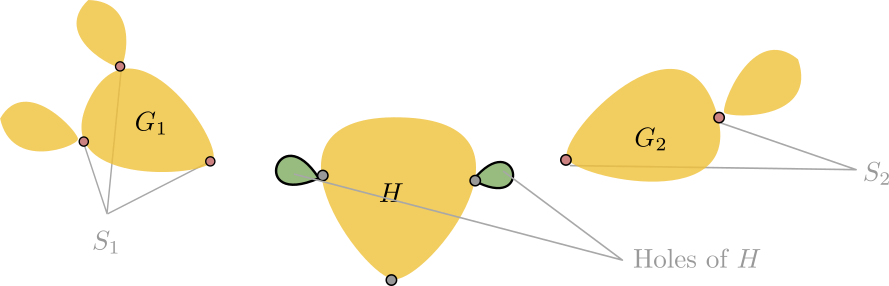
\includegraphics[scale=.36]{Pictures/decomp-test-proof}
\end{center}
By Lemma~\ref{lem:decomp-one-step}, the set of subgraphs $\cD$ defined below is an $L$-decomposition of $G$.
 $$\cD:=\cD_\mathsf{t}(S_1)\cup\dots\cup\cD_\mathsf{t}(S_k)\cup\set{G}$$
  To conclude we only need to find a set of vertices $S$ of $G$ such that $\cD_\mathsf{t}(S)=\cD$. Let $S=S_1\cup\dots\cup S_k\cup\set{\iota}$, where $\iota$ is the interface of $G$. Let us show that $\cD_\mathsf{t}(S)=\cD$. This is a consequence of the following lemma:

\begin{lemma}\label{lem-max-modules-context} Let $C$ be a context, $K$ a graph  and $I$ an interface in $H$ of the same arity as the hole of $C$. Suppose that the hole of $C$ is not parallel to any module. We have:
$$ \mathsf{max\text{-}module}_{\;C[K]}(I)=\mathsf{max\text{-}module}_{\;K}(I)$$
\end{lemma}
\begin{proof} Let $M:=\mathsf{max\text{-}module}_K(I)$.
Note that $M$ is a module of $G[K]$,  the question is its maximality. 
If $I$ is not the interface of $K$, then $M$ is maximal in  $G[K]$ because this substitution does not add any modules to $M$. 
Suppose that $I$ is the interface of $H$. In this case, we have $M=K$. Suppose by contradiction that there is a module $M'$ of  $G[K]$ strictly  containing  $K$ and whose interface is $I$. Hence, there is a module $M''$ such that $M'=(K\parallel M'')$. This means that $M''$ is module parallel to the hole of  $C$, which is not possible by hypothesis. 
\end{proof}
\end{proof}


\begin{theorem} 
Suppose that $\mu x. L$ is a guarded iteration of type test. We have: 
$$ L\text{ is $\CMSO$ definable} \quad \Rightarrow \quad  \mu x.L \text{ is  $\CMSO$ definable}$$
\end{theorem}

\begin{proof} Let $\phi$ be a $\CMSO$ formula whose language is $L$.
We transform the $\CMSOd$ formula $\mu x. \phi$ of Def.~\ref{def:iteration}, whose language is $\mu x. L$, into a $\CMSO$ formula  ${\mu x^g. \phi}$ of the same language. The formula ${\mu x^g. \phi}$ is obtained by replacing the quantification $\exists \cX.\ $ by the set quantification $\exists S.\ $, and by replacing every sub-formula of $\mu x. \phi$ of the form $(s,Z,t)\in \cX$ by this formula: 
$$(s=t) \ \wedge\ s\in S \ \wedge\ \text{``$(s,Z,t)$ is a maximal module''} $$
The last part of this formula is expressible in $\CMSO$ thanks to Prop.~\ref{prop:pure-modules-are-CMSO}. The language of ${\mu x^g. \phi}$ is the set of graphs for which we can find an $L$-decomposition encoded by a set of vertices $S$, and this is precisely the language $\mu x. L$ thanks to Prop.~\ref{prop:decomp-iteration-test}.
\end{proof}

\subsubsection{The case of domain  languages}
Let $\mu x. L$ be a guarded iteration of type \emph{domain}, $G$ a graph of $\mu x. L$ and $\cD$ an $L$-decomposition of $G$. Contrarily to the test case, the set of vertices  of $G$ corresponding to the interfaces of $\cD$, are not enough information to reconstruct $\cD$. Indeed, in this case,  a component of $\cD$ whose interface is $v$ is not necessarily the maximal module at $v$, but some domain module of interface $v$, among possibly many others. 
A way to determine if a domain module is in the decomposition is to check whether it contains an interface of the decomposition. This works for the components which are not the leaves of the decomposition. For the other components, we need to say explicitly which domain modules are the leaves. Since the later are pairwise independent, we can do so by coloring their inner edges and vertices. 



In the following, we show that a set of vertices of a graph (representing the interfaces of a decomposition) together with a coloring of this graph (indicating which modules are leaves), is enough to recover the decomposition. This justifies the following definitions.
 
\begin{definition}[Coloring, active modules.]
A \emph{coloring} of a graph $G$ is a set of its edges called \emph{leaf edges}. A module of $G$ is \emph{active} if it contains a leaf edge.

% A module is \emph{residual} if all its edges and inner vertices are residual; and \emph{principal} otherwise.
%
%\noindent Let $I$ be a pair of vertices in a graph. The \emph{maximal residual module at $I$} is the largest residual module whose interface is $I$.
\end{definition}
%\begin{remark}
%A module is principal if it contains \textbf{some} non-residual edge or  inner vertex.
%\end{remark}
%Given a set of vertices  $S$ and a coloring $\col$ of a graph $G$, we associate them with a set of subgraphs $\cD_\mathsf{d}(S, \col)$ as follows. 

\begin{definition}[$\cD_\mathsf{d}(S, \col)$] Let $G$ be a graph, $S$ a set of vertices and $\col$ a coloring of $G$.   

 \noindent We let $\cD_\mathsf{d}(S, \col)$ bet the set of active modules of $G$ of type $\mathsf{d}$, whose interfaces belong to $S$. 
\end{definition}

\begin{example}
\end{example}

\begin{proposition}\label{prop:decomp-iteration-dom} Let  $\mu x. L:\mathsf{d}$ be a guarded iteration. We have:
$$\begin{array}{rll}
 \quad G\in \mu x. L& \Leftrightarrow& \exists S, \col.\quad  S \text{ is a set of vertices and $\col$ a coloring of $G$ such that }\\
                      &             & \qquad\qquad \cD_\mathsf{d}(S,\col) \text{ is an $L$-decomposition of $G$.} 
\end{array}
$$
\end{proposition}

\begin{proof} 
The implication $(\Leftarrow)$ follows from Prop.~\ref{lem:decomp-iteration}. Let us prove the implication $(\Rightarrow)$.  Let $P_n$ be the following property:
$$\begin{array}{lrll}
P_n:&\ \forall G.\  G\in L^{n,x}& \Rightarrow& \exists S, \col.\quad  S \text{ is a set of vertices and $\col$ a coloring of $G$ such that }\\
 &                      &             & \qquad\qquad \cD_\mathsf{d}(S,\col) \text{ is an $L$-decomposition of $G$.} 
\end{array}
$$
We prove, by induction on $n$, that $P_n$ is valid for every $n\geq 1$, which  is enough to conclude. 
\medskip

 When $n=1$, we let $S$ be the singleton containing the interface of $G$ and  $\col$ be the coloring where all the edges of $G$ are leaves. We have $\cD_\mathsf{d}(S,\col)=\set{G}$, and since $G\in L$,   $\cD_\mathsf{d}(S,\col)$ is an $L$-decomposition of $G$.
\medskip

 Let $G\in L^{n+1,x}$. There are graphs $G_1, \dots, G_k$ and a $k$-context $H$ satisfying:
 $$G=H[G_1,\dots, G_k], \quad H[x,\dots,x]\in L\quad \text{ and }\quad  G_i\in L^{n,x} \text{ for } i\in[1,k].$$
 Let $S_i$ and $\col_i$ be the set of vertices and the coloring provided by induction hypothesis applied to $G_i$, for $i\in[1,k]$. 
 By Lemma~\ref{lem:decomp-one-step}, the set of subgraphs
 $$\cD:=\cD_\mathsf{d}(S_1,\col_1)\cup\dots\cup\cD_\mathsf{d}(S_k,\col_k)\cup\set{G}$$
 is an $L$-decomposition of $G$. To conclude we only need to find a set of vertices $S$ and a coloring $\col$ of $G$ such that $\cD_\mathsf{d}(S,\col)=\cD$. Let $\iota$ be the interface of $G$, and we set:
    $$S:=S_1\cup\dots\cup S_k\cup\set{\iota} \qquad\text{and}\qquad \col:=\col_1\cup\dots\cup \col_k$$
It is clear that $\cD_\mathsf{d}(S,\col)=\cD$.
\end{proof}

\begin{theorem} 
Suppose that $\mu x. L:\mathsf{d}$ be a guarded iteration. We have: 
$$ L\text{ is $\CMSO$ definable} \quad \Rightarrow \quad  \mu x.L \text{ is  $\CMSO$ definable}$$
\end{theorem}
\begin{proof} Let $\phi$ be a $\CMSO$ formula whose language is $L$.
We transform the $\CMSOd$ formula $\mu x. \phi$ of Def.~\ref{def:iteration}, whose language is $\mu x. L$, into a $\CMSO$ formula  $\mu x^g. \phi$ of the same language.  The formula $\mu x^g. \phi$ is obtained by replacing the quantification $\exists \cX.\ $ by the set quantifications $\exists S.\ \exists \mathsf{\col}.\ $, by saying that $\col$ is a set of edges and by replacing every sub-formula of $\mu x. \phi$ of the form $(s,Z,t)\in \cX$ by the following formula: 
$$(s=t) \ \wedge\ s\in S \ \wedge\ \text{``$(s,Z,t)$ is a module of type domain''} \ \wedge\  \text{``$(s,Z,t)$ is active''}$$
Being a module of type domain is expressible in $\CMSO$ thanks to Prop.~\ref{prop:pure-modules-are-CMSO}. Being active is  $\CMSO$ definable by the following formula:
$$ \exists x\in Z.\  x\in\col$$
The language of $\mu x^g. \phi$ is the set of graphs for which there is an $L$-decomposition encoded by a set of vertices $S$ and a coloring $\col$. This is precisely the language $\mu x. L$ by Prop.~\ref{prop:decomp-iteration-dom}.
\end{proof}

\subsubsection{The case of parallel languages}
The case of guarded iterations of type parallel is similar to the test case. Let $\mu x. L$ be a guarded iteration of type parallel, $G$ a graph of $\mu x. L$ and $\cD$ an $L$-decomposition of $G$. We show that the set of interfaces $I$ of $\cD$ is enough to recover the whole decomposition $\cD$, because its components are the maximal modules of $G$ whose interfaces belong to $I$. However, in this case,  the set of interfaces $I$ is no longer a set of vertices, but a set of pairs of vertices, that is a relation on the vertices of $G$. We will show that this relation is necessarily a companion relation. Using this result and the fact that $\CMSO$ and $\CMSO^r$ have the same expressive power, we prove that the iteration is $\CMSO$ definable. 

\begin{definition}[$\cD_\mathsf{p}(R)$] Let $G$ be a graph and $R$ a relation on the vertices of $G$.   
We define $\cD_\mathsf{p}(R)$ as the set of maximal modules of $G$, whose type is parallel, and whose interfaces belong to $S$.  
\end{definition}

\begin{proposition}\label{prop:decomp-iteration-parallel} Let  $\mu x. L$ be a guarded iteration of type parallel. We have:
$$\begin{array}{rll}
  G\in \mu x. L& \Leftrightarrow& \exists R.\quad  R \text{ is a set of vertices of $G$ and }\\
                      &             & \qquad \cD_\mathsf{p}(R) \text{ is an $L$-decomposition of $G$.} 
\end{array}
$$
\end{proposition}

\begin{proof} 
$(\Rightarrow)$ Follows from Prop.~\ref{lem:decomp-iteration}. To prove $(\Leftarrow)$, we let $P_n$ be the following property:
$$
\begin{array}{llll}
\forall G.\quad G\in L^{n,x}& \Rightarrow & \exists R.\quad  R \text{ is a relation on the vertices of $G$ and }\\  
&&  \qquad \cD_\mathsf{p}(R) \text{ is an $L$-decomposition of $G$.}
\end{array}
$$
We prove, by induction on $n$, that $P_n$ is valid for every $n\geq 1$, and this is enough to conclude. 
\smallskip

 When $n=1$, take $R$ to be the singleton containing the interface of $G$. We have that $\cD_\mathsf{p}(R)=\set{G}$ and since $G\in L$, we have that $\cD_\mathsf{p}(R)$ is an $L$-decomposition of $G$.
\medskip

 Let $G\in L^{n+1,x}$. There is a $k$-context $H$ and  graphs $G_1, \dots, G_k$ such that: 
$$G=H[G_1,\dots, G_k],\quad H[x,\dots,x]\in L\quad \text{ and }\quad G_i\in L^{n,x}, \text{ for } i\in[1,k].$$ 
Thanks to the guard condition, the holes of $H$ have no parallel modules.  For every $i\in[1, k]$, let $R_i$ be the relation provided by the induction hypothesis applied to the graph $G_i$. By Lemma~\ref{lem:decomp-one-step}, the following set of subgraphs:
 $$\cD:=\cD_\mathsf{p}(R_1)\cup\dots\cup\cD_\mathsf{p}(R_k)\cup\set{G}$$
 is an $L$-decomposition of $G$. To conclude we only need to find a relation $R$ on the vertices of $G$ such that $\cD_\mathsf{p}(R)=\cD$. If $I$ is the interface of $G$, we let $R$ to be the following relation:
  $$R=R_1\cup\dots\cup R_k\cup\set{I}$$ 
  The fact that $\cD_\mathsf{t}(S)=\cD$ is a consequence of lemma~\ref{lem-max-modules-context}.
\end{proof}

\begin{proposition}\label{prop:interface-are-comp-parallel}
Let $\mu x. L$ be an iteration of type parallel and let $G$ a graph. The interfaces of every $L$-decomposition of $G$ form a companion relation.
\end{proposition}

\begin{proof}
We prove by induction on $n\geq 1$ that the interfaces of every $L$-decomposition  of depth $n$ of some graph $G$ form a companion relation, witnessed by a set of paths $P$, such that the interface of $G$ is witnessed by two parallel paths of $P$. 
\medskip

 When $n=1$, the decomposition $\cD$ is reduced to the graph $G$. Since $G$ is parallel, it has two parallel paths whose interface is the interface of $G$. Take $P$ to be these two paths. 
\medskip

Suppose that $\cD$ is a decomposition of depth $n+1$. Hence it is of the form: 
$$\cD=\cD_1\cup\dots\cD_k\cup\set{G}$$ 
where $\cD_i$ is an $L$-decomposition of depth at most $n$, of a graph $G_i$, for every $i\in[1,k]$. Let $P_i$ be the set of paths provided by the induction hypothesis for $\cD_i$, and let $p_i, q_i$ be the two paths witnessing the interface of $G_i$, for $i\in[1,k]$.
\medskip

We set $H: = x$-$\mathsf{body}_\cD(G)$.  Since $H$ is parallel, it has two parallel paths $p$ and $q$ whose interface is the interface of $H$. We transform the paths $p$ and $q$ of $H$ into the paths $p'$ and $q'$ of $G$ as follows. The paths $p'$ and $q'$ are obtained from $p$ and $q$ respectively by the following procedure: if $e$ is an $x$-edge of $H$ which is substituted by some $G_i$, then replace $e$ by the path of $p_i$. Let $P$ be the following set of paths: $$P=(P_1\setminus\set{p_1})\cup\dots (P_k\setminus\set{p_k}) \cup\set{p',q'}.$$
 The set $P$ is orthogonal and witnesses the interfaces of $\cD$. Moreover, the interface of $G$ is witnessed by two parallel paths of $P$, namely $p'$ and $q'$. This concludes the proof.
\end{proof}
\begin{remark}
We do not need the guard condition for Prop.~\ref{prop:interface-are-comp-parallel}.
\end{remark}

\begin{corollary}\label{cor:decomp-iteration-parallel}
Let  $\mu x. L$ be a guarded iteration of type parallel. We have:
$$\begin{array}{rll}
  G\in \mu x. L& \Leftrightarrow& \exists R.\quad  R \text{ is a companion relation on the vertices of $G$ and }\\
                      &             & \quad\quad\   \cD_\mathsf{p}(R) \text{ is an $L$-decomposition of $G$.} 
\end{array}
$$
\end{corollary}

\begin{theorem} 
Suppose that $\mu x. L$ is a guarded iteration of type parallel. We have: 
$$ L\text{ is $\CMSO$ definable} \quad \Rightarrow \quad  \mu x.L \text{ is  $\CMSO$ definable}$$
\end{theorem}

\begin{proof} Let $\phi$ be a $\CMSO$ formula whose language is $L$.
We will transform the $\CMSOd$ formula $\mu x. \phi$ of Def.~\ref{def:iteration}, whose language is $\mu x. L$, into a $\CMSO^r$ formula  ${\mu x^r. \phi}$ of the same language. The formula ${\mu x^r. \phi}$ is obtained by replacing the quantification $\exists \cX\ $ by the set quantification $\exists R\ $, and by replacing every sub-formula of $\mu x. \phi$ of the form $(s,Z,t)\in \cX$ by the following formula: 
$$ (s,t) \in R \ \wedge\ \text{``$(s,Z,t)$ is a maximal module''} $$
The last part of this formula is expressible in $\CMSO$ thanks to Prop.~\ref{prop:pure-modules-are-CMSO}.  The language of ${\mu x^r. \phi}$ is the set of graphs for which we can find an $L$-decomposition encoded by a companion relation $R$, and this is precisely the language $\mu x. L$ thanks to Cor.~\ref{cor:decomp-iteration-parallel}. Since $\CMSO^r$ and $\CMSO$ have the same expressive power, this concludes the proof.
\end{proof}


\subsubsection{The case of series languages}
Let $\mu x. L$ be a guarded iteration of type series, $G$ a graph in $\mu x. L$ and $\cD$ an $L$-decomposition of $G$ whose set of interfaces is $I$. As for the domain case, the set $I$ is not enough to reconstruct the decomposition $\cD$, and we need a coloring of the graph to determine which modules are the leaves of the decomposition $\cD$. We show also that the set of interfaces $I$ is a companion relation, which will be enough to conclude. 
%Given a set of vertices  $S$ and a coloring $\col$ of a graph $G$, we associate them with a set of subgraphs $\cD_\mathsf{d}(S, \col)$ as follows. 

\begin{definition}[$\cD_\mathsf{s}(R, \col)$] Let $G$ be a graph, $R$ a relation on the vertices of $G$ and $\col$ a coloring of $G$.  We let $\cD_\mathsf{s}(R, \col)$ bet the set of active modules of $G$ of type series, whose interfaces belong to $R$. 
\end{definition}


\begin{proposition}\label{prop:decomp-iteration-series} Let  $\mu x. L$ be a guarded iteration of type series. We have:
$$\begin{array}{rll}
 \quad G\in \mu x. L&  \qquad\Leftrightarrow \qquad& \exists R, \col.\quad  R \text{ is a relation on the vertices of $G$,}\\
 					&           & \qquad\qquad \text{$\col$ is a coloring of $G$ and}\\
                      &             & \qquad\qquad \cD_\mathsf{s}(R,\col) \text{ is an $L$-decomposition of $G$.} 
\end{array}
$$
\end{proposition}

\begin{proof} 
$(\Leftarrow)$ Follows from Prop.~\ref{lem:decomp-iteration}. To prove  $(\Rightarrow)$, we let $P_n$ be the following property:
$$\begin{array}{rll}
 \forall G. \quad G\in L^{n,x}& \Leftrightarrow& \exists R, \col.\quad  R \text{ is a relation on the vertices of $G$,}\\
 					&           & \qquad\qquad \text{$\col$ is a coloring of $G$ and}\\
                      &             & \qquad\qquad \cD_\mathsf{s}(R,\col) \text{ is an $L$-decomposition of $G$.} 
\end{array}
$$
We prove, by induction on $n$, that $P_n$ is valid for every $n\geq 1$, which  is enough to conclude. 
\medskip

 When $n=1$, let $R$ be the singleton containing the interface of $G$ and let $\col$ be the coloring where all the edges of $G$ are leaves. We have $\cD_\mathsf{s}(R,\col)=\set{G}$, and since $G\in L$,   $\cD_\mathsf{s}(R,\col)$ is an $L$-decomposition of $G$.
\medskip

 Let $G\in L^{n+1,x}$. There are graphs $G_1, \dots, G_k$ and a $k$-context $H$ satisfying:
 $$G=H[G_1,\dots, G_k], \quad H[x,\dots,x]\in L\quad \text{ and }\quad  G_i\in L^{n,x} \text{ for } i\in[1,k].$$
 Let $R_i$ and $\col_i$ be the relation and the coloring provided by induction hypothesis applied to $G_i$, for $i\in[1,k]$. 
 By Lemma~\ref{lem:decomp-one-step}, the following set of subgraphs:
 $$\cD:=\cD_\mathsf{s}(R_1,\col_1)\cup\dots\cup\cD_\mathsf{s}(R_k,\col_k)\cup\set{G}$$
 is an $L$-decomposition of $G$. To conclude we only need to find a relation $R$ on the vertices of $G$ and a coloring $\col$ of $G$ such that $\cD_\mathsf{d}(S,\col)=\cD$. Let $I$ be the interface of $G$, we set:
    $$R:=R_1\cup\dots\cup R_k\cup\set{I}\qquad \text{and}\qquad \col:=\col_1\cup\dots\cup \col_k.$$
The fact that $\cD_\mathsf{d}(S,\col)=\cD$ is a consequence of following easy lemma:
\begin{lemma}
If $C$ is a context, $K$ a graph of interface $J$ and $I$ an interface in $K$, then:
$$\begin{array}{llr}
\mathsf{series\text{-}modules}_{\;C[K]}(I)&=\mathsf{series\text{-}modules}_{\;K}(I) & \text{ if }\quad I\neq J, \\
&=\mathsf{series\text{-}modules}_{\;K}(I)\cup \mathsf{series\text{-}modules}_{\;\overline{C}}(I)  & \text{ if }\quad  I=J.
\end{array} $$
Where $\overline{C}$ is the context $C$ without its hole.
\end{lemma}
\end{proof}

\begin{proposition}\label{prop:interface-are-comp-series}
Let $\mu x. L$ be a guarded iteration of type series and let $G$ be a graph. The interfaces of every $L$-decomposition of $G$ form a companion relation.
\end{proposition}

\begin{proof} We start by proving the following claim:
\begin{claim}\label{new-claim-series}
Let $H$ be a pure binary graph of interface $I$ and suppose that $x$ is $\mathsf{s}$-guarded in $H$. There is a path $p$ in $H$ of interface $I$, such that every  $x$-edge of $p$ is a parallel to an $x$-edge in $H$. 
%If $H$ is a pure binary graph and $x$ is not in a series context in $H$, then there is a path $p$ from the input to the output of $H$, such that for any edge $s\fleche{x}t$ in $p$, there is a parallel edge $s\fleche{x}t$ in $H$.%  is an $x$-edge of $p$, then there is another x-edge $e'$ of $H$ with the same interface as $e$.
\end{claim}
\begin{proof}
We proceed by induction on the size of $H$. The case where $H$ is atomic is trivial.

 
If $H$ is series, then we can write $H$ under the following form:
 $$H=U_0\cdot P_1\cdot U_1\cdot P_1\dots U_{k-1}\cdot P_k\cdot U_k$$
  where $P_i$ is a parallel graph and $U_j$ a unary graph for every $i\in[1,k]$ and $j\in[0,k]$.
  For every $i\in[1,k]$, $x$ is $\mathsf{s}$-guarded in $P_i$, otherwise $x$ would not be guarded in $H$. For every $i\in [1,k]$, the induction hypothesis applied to $P_i$ provides us with a path $p_i$. We let $p$ be the concatenation of the paths $p_i$, for $i\in[1,k]$. The path $p$ satisfies the required condition.
\medskip

If $H$ is parallel, then we can write $H$ under the following form:
$$H=H_1\parallel\dots \parallel H_k$$
 where for every $i\in [1,k]$, the graph $H_i$ is either $(1)$ a series graph which is not the graph of the letter $x$, or $(2)$ the graph of the letter $x$.

If there is $j\in[1,k]$ satisfying $(1)$, then the letter $x$ is $\mathsf{s}$-guarded in $H_j$. We can conclude by induction hypothesis. Otherwise, for all $j\in[1,k]$, $H_j$ is the graph of the letter $x$. Any path from the the input to the output of $H$ satisfies the condition of the claim. 
 \end{proof}
 We prove by induction on $n\geq 1$ that the interfaces of every $L$-decomposition  of depth $n$ of some graph $G$ form a companion relation, witnessed by a safe set of paths $P$. 
\medskip

 When $n=1$, the decomposition $\cD$ is reduced to the graph $G$. Since $G$ is series, it has a path whose interface is the interface of $G$. Take $P$ to be the set containing this path. 
\medskip

 Suppose that $\cD$ is a decomposition of depth $n+1$. Hence it is of the form: 
$$\cD=\cD_1\cup\dots\cD_k\cup\set{G}$$ 
where $\cD_i$ is an $L$-decomposition of depth at most $n$ of a graph $G_i$, for every $i\in[1,k]$. Let $P_i$ be the set of paths provided by the induction hypothesis for $\cD_i$ for $i\in[1,k]$.
\medskip

We set $H=x$-$\mathsf{body}_\cD(G)$.  Since $x$ is $\mathsf{s}$-guarded in $H$, the Claim~\ref{new-claim-series} provides us with a path $p$. We transform the path $p$ of $H$ into the path $p'$ of $G$ as follows. The path $p'$ is obtained from $p$ as follows: if $e$ is an $x$-edge of $H$ which is substituted by a graph $G_i$, for some $i\in [1,k]$, then replace $e$ by the path $p_i$ witnessing the interface of $G_i$. We denote by $Q$ the set of paths $p_i$ which participated to this procedure. 
 Let $P$ be the following set of paths: $$P=P_1\cup\dots \cup P_k\cup\set{p'}\setminus Q.$$
 The set $P$ is safe, orthogonal and witnesses the interfaces of $\cD$.  This concludes the proof.

\end{proof}
\begin{remark}
Contrarily to Prop.~\ref{prop:interface-are-comp-parallel}, we need the guard condition to prove Prop.~\ref{prop:interface-are-comp-series}.
\end{remark}

\begin{corollary}\label{cor:decomp-iteration-series}
Let  $\mu x. L$ be a guarded iteration of type parallel. We have:
$$\begin{array}{rll}
  G\in \mu x. L& \Leftrightarrow& \exists R.\ \col. \quad  R \text{ is a companion relation on the vertices of $G$,}\\
                        &             & \qquad\qquad\   \col \text{ is a coloring of $G$ and } \\
                      &             & \qquad\qquad\   \cD_\mathsf{s}(R,\col) \text{ is an $L$-decomposition of $G$.} 
\end{array}
$$
\end{corollary}

\begin{theorem} 
Suppose that $\mu x. L$ is a guarded iteration of type series. We have: 
$$ L\text{ is $\CMSO$ definable} \quad \Rightarrow \quad  \mu x.L \text{ is  $\CMSO$ definable}$$
\end{theorem}
\begin{proof} Let $\phi$ be a $\CMSO$ formula whose language is $L$.
We will transform the $\CMSOd$ formula $\mu x. \phi$ of Def.~\ref{def:iteration}, whose language is $\mu x. L$, into a $\CMSO^r$ formula  $\mu x^r. \phi$ of the same language.  The formula $\mu x^r. \phi$ is obtained by replacing the quantification $\exists \cX$ by the set quantifications $\exists R.\ \exists \col.\ $, expressing that $\col$ is a set of edges and by replacing every sub-formula of $\mu x. \phi$ of the form $(s,Z,t)\in \cX$ by the following formula: 
$$(s=t) \ \wedge\ s\in S \ \wedge\ \text{``$(s,Z,t)$ is a module of type series''} \ \wedge\  \text{``$(s,Z,t)$ is active''}$$
Being a module of type series is expressible in $\CMSO$ thanks to Prop.~\ref{prop:pure-modules-are-CMSO}. Being active is  $\CMSO$ definable by the following formula:
$$ \exists x\in Z.\  x\in\col$$
The language of $\mu x^r. \phi$ is the set of graphs for which we can find an $L$-decomposition encoded by a companion relation $R$ and a coloring $\col$, and this is precisely the language $\mu x. L$ thanks to Prop.~\ref{prop:decomp-iteration-series}.
\end{proof}